\chapter{Lateral pile capacity (Full plastification)}\label{sec_7}

The lateral pile capacity is checked in accordance to both BSH, cf. Figure ~\ref{BSH}, and in accordance to DNVGL, cf. Figure ~\ref{DNV}. For the BSH check a resistance factor of 1.4 is applied to the resistance side of the soil springs, while for the DNVGL check the soil strength parameters are reduced by a material factor of 1.25. For both checks the utilization is below unity showing that the foundation has sufficient capacity against lateral loading.

\begin{figure}[!htbp]
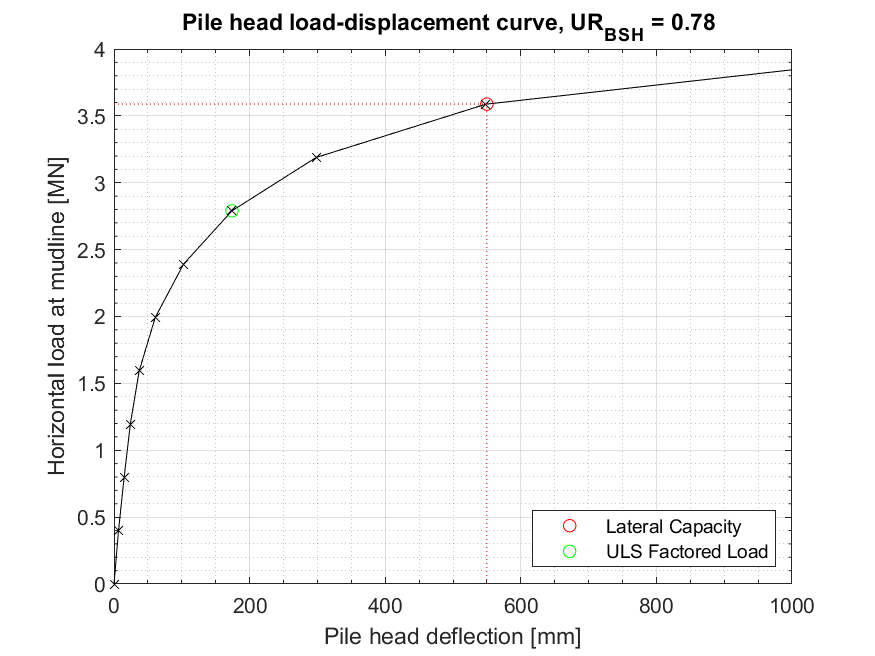
\includegraphics[width=0.9\textwidth]{AppendixGenerationFiles/ProjectLocation/utilization_ratio_BSH.png}
\caption{Lateral load-deflection curve, lateral capacity for BSH regulations, factored ULS loading at mudline, and utilization ratio (UR) at WTG {\ID_location}. Characteristic soil properties and with resistance factor applied to soil springs.}
\label{BSH}\end{figure}


\begin{figure}[!htbp]
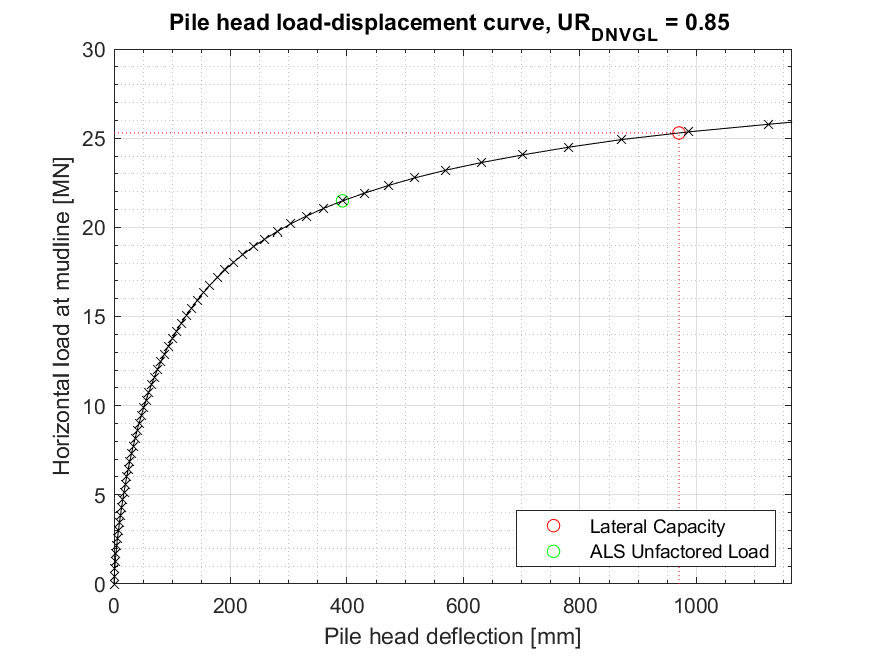
\includegraphics[width=0.9\textwidth]{AppendixGenerationFiles/ProjectLocation/utilization_ratio_DNV.png}
\caption{Lateral load-deflection curve, lateral capacity for DNVGL regulations, factored ULS loading at mudline, and utilization ratio (UR) at WTG {\ID_location}. Characteristic soil properties, but with material factor of 1.25 applied to undrained shear strength.}
\label{DNV}\end{figure}